\hypertarget{group__slipif}{}\section{S\+L\+IP netif}
\label{group__slipif}\index{S\+L\+I\+P netif@{S\+L\+I\+P netif}}
Collaboration diagram for S\+L\+IP netif\+:
\nopagebreak
\begin{figure}[H]
\begin{center}
\leavevmode
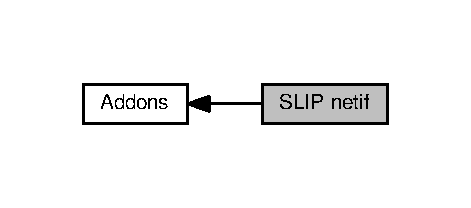
\includegraphics[width=226pt]{group__slipif}
\end{center}
\end{figure}
This is an arch independent S\+L\+IP netif. The specific serial hooks must be provided by another file. They are sio\+\_\+open, sio\+\_\+read/sio\+\_\+tryread and sio\+\_\+send

Usage\+: This netif can be used in three ways\+:~\newline
 1) For N\+O\+\_\+\+S\+YS==0, an RX thread can be used which blocks on \hyperlink{native_2lwip_2src_2include_2lwip_2sio_8h_ac5a6563ee5f12459451010139a04a03b}{sio\+\_\+read()} until data is received.~\newline
 2) In your main loop, call \hyperlink{native_2lwip_2src_2netif_2slipif_8c_a7b036fd1cde9b299139cac62f52d15a6}{slipif\+\_\+poll()} to check for new RX bytes, completed packets are fed into netif-\/$>$input().~\newline
 3) Call slipif\+\_\+received\+\_\+byte\mbox{[}s\mbox{]}() from your serial RX I\+SR and slipif\+\_\+process\+\_\+rxqueue() from your main loop. I\+SR level decodes packets and puts completed packets on a queue which is fed into the stack from the main loop (needs S\+Y\+S\+\_\+\+L\+I\+G\+H\+T\+W\+E\+I\+G\+H\+T\+\_\+\+P\+R\+OT for pbuf\+\_\+alloc to work on I\+SR level!). 